\documentclass{llncs}
\usepackage{url}
\usepackage{proof}
\usepackage{amssymb}
\usepackage{stmaryrd}
\usepackage{listings}
\usepackage{graphicx}

%subcode-inline{bnf-inline} name langRev
%! swap+ = \mathit{swap}^+
%! swap* = \mathit{swap}^*
%! dagger =  ^{\dagger}
%! assocl+ = \mathit{assocl}^+
%! assocr+ = \mathit{assocr}^+
%! assocl* = \mathit{assocl}^*
%! assocr* = \mathit{assocr}^*
%! identr* = \mathit{uniti}
%! identl* = \mathit{unite}
%! dist = \mathit{distrib}
%! factor = \mathit{factor}
%! (o) = \fatsemi
%! (;) = \fatsemi
%! (*) = \times
%! (+) = +


%subcode-inline{bnf-inline} regex \{\{(((\}[^\}])|[^\}])*)\}\} name main include langRev
%! [^ = \ulcorner
%! ^] = \urcorner
%! [v = \llcorner
%! v] = \lrcorner
%! |-->* = \mapsto^{*}
%! |-->> = \mapsto_{\ggg}
%! |-->let = \mapsto_{let}
%! |--> = \mapsto
%! <--| = \mapsfrom
%! |- = \vdash
%! in = \!\!\in\!\!
%! <=> = \Longleftrightarrow
%! <-> = \leftrightarrow
%! ~> = \leadsto
%! ::= = ::=
%! /= = \neq
%! vi = v_i
%! di = d_i
%! si = s_i
%! sj = s_j
%! F = \texttt{F}
%! T = \texttt{T}
%! forall = \forall
%! exists = \exists
%! empty = \emptyset
%! eta = \eta
%! where = \textbf{where}
%! epsilon = \varepsilon
%! least = \phi
%! trace+ = trace
%! trace* = trace_{\times}
%! loop+ = loop_{+}
%! loop* = loop_{\times}
%! CatC = {\mathcal C}
%! CatA = {\mathcal A}
%! gamma = \gamma
%! {[ = \{
%! ]} = \}
%! elem = \in
%! dagger = ^\dagger
%! alpha = \alpha
%! beta = \beta
%! rho = \rho
%! @@ = \mu
%! @ = \,@\,
%! * = \times
%! langRev = \Pi
%! langRevT = \Pi^{o}
%! langRevEE = \Pi^{\eta\epsilon}_{+}
%! bullet = \bullet

\urldef{\mails}\path|{rpjames, sabry}@indiana.edu|

%%%%%%%%%%%%%%%%%%%%%%%%%%%%%%%%%%%%%%%%%%%%%%%%%%%%%%%%%%%%%%%%%%%%%%%%%%%%%

\begin{document}
\title{Isomorphic Interpreters from Logically Reversible Abstract Machines} 
\titlerunning{On the Construction of Isomorphic Interpreters} 
\author{Roshan P. James \and Amr Sabry}
\institute{School of Informatics and Computing, Indiana University\\
\mails}
\maketitle

%%%%%%%%%%%%%%%%%%%%%%%%%%%%%%%%%%%%%%%%%%%%%%%%%%%%%%%%%%%%%%%%%%%%%%%%%%%%%
\begin{abstract}
% Previous work on {{langRevT}} \cite{rc2011,infeffects} studied its
% properties and various constructions in it. However, for a
% computational model, there has been little focus on actually writing
% programs directly in {{langRevT}}. This paper aims to remedy that by
% presenting a systematic technique of expressing logically reversible
% small-step abstract machines in {{langRevT}}. In other words, this
% paper shows that once we have a logically reversible machine in a
% notation of our choice, expressing the machine as an isomorphic
% interpreter in {{langRevT}} can be done systematically and does not
% present any significant conceptual difficulties. This gives us a means
% of developing large {{langRevT}} programs with the ease of reasoning
% at the level of a conventional small-step semantics.  We develop
% several simple interpreters over numbers and addition, move onto tree
% traversal and finish with an interpreter for {{langRevT}} expressed in
% {{langRevT}}.
  In our previous work, we developed a reversible programming language and
  established that every computation in it is a (partial) isomorphism that is
  reversible and that preserves information. The language is founded on type
  isomorphisms that have a clear categorical semantics but that are awkward
  as a notation for writing actual programs, especially recursive ones. This
  paper remedies this aspect by presenting a systematic technique for
  developing a large and expressive class of reversible recursive programs,
  that of logically reversible small-step abstract machines. In other words,
  this paper shows that once we have a logically reversible machine in a
  notation of our choice, expressing the machine as an isomorphic interpreter
  can be done systematically and does not present any significant conceptual
  difficulties. Concretely, we develop several simple interpreters over
  numbers and addition, move on to tree traversals, and finish with a
  meta-circular interpreter for our reversible language. This
  gives us a means of developing large reversible programs with the ease of
  reasoning at the level of a conventional small-step semantics.
\end{abstract}


%%%%%%%%%%%%%%%%%%%%%%%%%%%%%%%%%%%%%%%%%%%%%%%%%%%%%%%%%%%%%%%%%%%%%%%%%%%%%
\section{Introduction} 

In recent papers~\cite{rc2011,James:2012:IE:2103656.2103667}, we developed a
pure reversible model of computation that is obtained from the type
isomorphisms and categorical structures that underlie models of linear logic
and quantum computing and that treats information as a linear resource that
can neither be erased nor duplicated. From a programming perspective, our
model gives rise to a pure (with no embedded computational effects such as
assignments) reversible programming language {{langRevT}} based on
\emph{partial isomorphisms}. In more detail, in the recursion-free fragment
of {{langRevT}}, every program witnesses an isomorphism between two finite
types; in the full language with recursion, some of these isomorphisms may be
partial, i.e., may diverge on some inputs. 

In this paper, we investigate the practicality of writing large recursive programs
in {{langRevT}}. Specifically, we assume that we are given some reversible
recursive algorithm expressed as a \emph{reversible abstract machine}, and we
show via a number of systematic steps, how to develop a {{langRevT}} program
from that abstract machine. Our choice of starting from reversible abstract
machines is supported by the following observations:
\begin{itemize}
\item it is an interesting enough class of reversible programs: researchers
  have invested the effort in manually designing such machines, e.g., the
  SE(M)CD machine~\cite{Kluge:1999:SEMCD}, and the SECD-H~\cite{lorenz};
\item every reversible interpreter can be realized as such a machine: this
  means that our class of programs includes self-interpreters which are
  arguably a measure of the strength of any reversible
  language~\cite{Axelsen:2011:RPC:1987171.1987176,Yokoyama:2008:PRP,Yokoyama:2007:RPL:1244381.1244404};
\item general recursive programs can be systematically transformed to
  abstract machines: the technique is independent of reversible programs and
  consists of transforming general recursion to tail recursion and then
  applying \emph{fission} to split the program into a driver and a small-step
  machine~\cite{Danvy:2008:RRN:1813347.1813350,Rendel:2010:ISD:1863523.1863525}.
\end{itemize}

To summarize, we assume we are given some reversible abstract machine and we
show how to derive a {{langRevT}} program that implements the semantics of
the machine. Our derivation is systematic and expressive. In particular,
{{langRevT}} can handle machines with stuck states because it is based on
partial isomorphisms. We illustrate our techniques with simple machines that
do bounded iteration on numbers, tree traversals, and a meta-circular
interpreter for {{langRevT}}. 

% To understand the problem in more detail, consider the problem of converting
% a reversible recursive function into a partial isomorphism. In general such a
% function takes an input, makes several recursive calls, and produces an
% answer. To implement this in a reversible way, the structure of the recursion
% and the number of recursive calls need to be exposed. The key trick is to
% express tease the function into two components: an outer driver that performs
% iteration and an inner state transition function that realizes one
% ``unfolding'' of the recursion. In program transformation world, this is
% called, light-weight fission. Using this idea, one can realize any recursive
% function as a partial isomorphism. We show a few examples of the construction
% culminating with the most challenging recursive function: a full interpreter.

% Previous work on {{langRevT}} \cite{rc2011,James:2012:IE:2103656.2103667}
% studied its properties and various constructions in it. However, for a
% computational model, there has been little focus on actually writing programs
% directly in {{langRevT}}. This paper aims to remedy that by presenting a
% systematic technique of expressing logically reversible small-step abstract
% machines in {{langRevT}}. This paper shows that once we have a logically
% reversible machine in a notation of our choice, expressing the machine as an
% isomorphic interpreter in {{langRevT}} can be done systematically and does
% not present any significant conceptual difficulties.

%% - write program; derive inverse
%% program~\cite{Gluck:2005,Mu:2002:IFF:648086.757330,conf/aplas/GluckK03,Gluck:2005};
%% we're not interested in this; we want to directly write partial isomorphisms

%%%%%%%%%%%%%%%%%%%%%%%%%%%%%%%%%%%%%%%%%%%%%%%%%%%%%%%%%%%%%%%%%%%%%%%%%%%%%%%%
\section{Review of the Reversible Language: {{langRevT}} }
\label{sec:pi}

We briefly review the reversible language {{langRevT}} introduced in our
previous work~\cite{rc2011,James:2012:IE:2103656.2103667}. The set of types
includes the empty type {{0}}, the unit type {{1}}, sum types {{b1+b2}},
product types {{b1*b2}}, and recursive types {{@@x.b}}. The set of values
{{v}} includes {{()}} which is the only value of type {{1}}, {{left v}} and
{{right v}} which inject {{v}} into a sum type, {{(v1,v2)}} which builds a
value of product type, and  which is used to construct recursive
values. There are no values of type {{0}}:
%subcode{bnf} include main
% value types, b ::= 0 | 1 | b + b | b * b | x | @@x.b
% values, v ::= () | left v | right v | (v, v) | <v>

The expressions of {{langRevT}} are witnesses to the following type
isomorphisms:
%subcode{bnf} include main
%! columnStyle = r@{\hspace{-0.5pt}}c@{\hspace{-0.5pt}}l
%zeroe :&  0 + b <-> b &: zeroi
%swap+ :&  b1 + b2 <-> b2 + b1 &: swap+
%assocl+ :&  b1 + (b2 + b3) <-> (b1 + b2) + b3 &: assocr+
%identl* :&  1 * b <-> b &: identr*
%swap* :&  b1 * b2 <-> b2 * b1 &: swap*
%assocl* :&  b1 * (b2 * b3) <-> (b1 * b2) * b3 &: assocr*
%dist0 :& 0 * b <-> 0 &: factor0
%dist :&~ (b1 + b2) * b3 <-> (b1 * b3) + (b2 * b3)~ &: factor
%fold :&~ b[@@x.b/x] <-> @@x.b ~&: unfold
Each line of the above table introduces one or two combinators that witness
the isomorphism in the middle. Collectively the isomorphisms state that the
structure {{(b,+,0,*,1)}} is a \emph{commutative semiring}, i.e., that each
of {{(b,+,0)}} and {{(b,*,1)}} is a commutative monoid and that
multiplication distributes over addition. The last isomorphism witnesses the
equivalence of a value of recursive type with all its ``unrollings.'' The
isomorphisms are extended to form a congruence relation by adding the
following constructors that witness equivalence and compatible closure. In
addition, the language includes a {{trace}} operator to express looping:
%subcode{proof} include main
%@  ~
%@@ id : b <-> b 
%
%@ c : b1 <-> b2
%@@ sym c : b2 <-> b1
%
%@ c1 : b1 <-> b2
%@ c2 : b2 <-> b3
%@@ c1(;)c2 : b1 <-> b3
%---
%@ c1 : b1 <-> b3
%@ c2 : b2 <-> b4
%@@ c1 (+) c2 : b1 + b2 <-> b3 + b4
%
%@ c1 : b1 <-> b3
%@ c2 : b2 <-> b4
%@@ c1 (*) c2 : b1 * b2 <-> b3 * b4
%
%@ c : b1 + b2 <-> b1 + b3
%@@ trace c : b2 <-> b3

\paragraph*{Adjoint.} 
An important property of the language is that every combinator {{c}} has an
adjoint {{c{dagger}}} that reverses the action of {{c}}. This is evident by
construction for the primitive isomorphisms. For the closure combinators, the
adjoint is homomorphic except for the case of sequencing in which the order
is reversed, i.e., {{(c1 (;) c2){dagger} = (c2{dagger}) (;) (c1{dagger}) }}.

\paragraph*{Graphical Language.}
Following the tradition for computations in monoidal
categories~\cite{springerlink:10.1007/978-3-642-12821-94}, we present a
graphical notation that conveys the semantics of {{langRevT}}.  The general
idea of the graphical notation is that combinators are modeled by ``wiring
diagrams'' or ``circuits'' and that values are modeled as ``particles'' or
``waves'' that may appear on the wires. Evaluation therefore is modeled by
the flow of waves and particles along the wires.

\begin{itemize}
\item The simplest sort of diagram is the {{id : b <-> b}} combinator which
  is simply represented as a wire labeled by its type {{b}}, as shown below
  on the left. In more complex diagrams, if the type of a wire is obvious
  from the context, it may be omitted. When tracing a computation, one might
  imagine a value {{v}} of type {{b}} on the wire, as shown below on the
  right:

  \begin{multicols}{2}
\begin{center}
\scalebox{0.95}{
%%subcode-line{pdfimage}[diagrams/thesis/b-wire.pdf]
\includegraphics{diagrams/thesis/b-wire.pdf}
}
\end{center}
\begin{center}
\scalebox{0.95}{
%%subcode-line{pdfimage}[diagrams/thesis/b-wire.pdf]
\includegraphics{diagrams/thesis/b-wire-value.pdf}
}
\end{center}
  \end{multicols}

\item The product type {{b1*b2}} may be represented using either one wire
  labeled {{b1*b2}} or two parallel wires labeled {{b1}} and {{b2}}. In the
  case of products represented by a pair of wires, when tracing execution
  using particles, one should think of one particle on each wire or
  alternatively as in folklore in the literature on monoidal categories as a
  ``wave:''
\begin{multicols}{4}
\begin{center}
\scalebox{0.95}{
%%subcode-line{pdfimage}[diagrams/thesis/pair-one-wire.pdf]
\includegraphics{diagrams/thesis/product-one-wire.pdf}
}
\end{center}
\columnbreak
\begin{center}
\scalebox{0.95}{
\includegraphics{diagrams/thesis/product-one-wire-value.pdf}
}
\end{center}
%% \end{multicols}
%% \begin{multicols}{2}
\begin{center}
\scalebox{0.95}{
%%%subcode-line{pdfimage}[diagrams/thesis/pair-of-wires.pdf]
\includegraphics{diagrams/thesis/product-two-wires.pdf}
}
\end{center}
\begin{center}
\scalebox{0.95}{
\includegraphics{diagrams/thesis/product-two-wires-value.pdf}
}
\end{center}
\end{multicols}

\item Sum types may similarly be represented by one wire or using parallel
  wires with a {{+}} operator between them. When tracing the execution of two
  additive wires, a value can reside on only one of the two wires:
\begin{multicols}{4}
%\begin{center}
\scalebox{0.95}{
%%subcode-line{pdfimage}[diagrams/thesis/sum-one-wire.pdf]
\includegraphics{diagrams/thesis/sum-one-wire.pdf}
}

%\end{center}
%% \end{multicols}
%% \begin{multicols}{2}
%\begin{center}
\scalebox{0.95}{
%%subcode-line{pdfimage}[diagrams/thesis/sum-of-wires.pdf]
\includegraphics{diagrams/thesis/sum-two-wires.pdf}
}

%\end{center}
%\begin{center}
\scalebox{0.95}{
\includegraphics{diagrams/thesis/sum-two-wires-left-value.pdf}
}

%\end{center}
%\begin{center}
\scalebox{0.95}{
\includegraphics{diagrams/thesis/sum-two-wires-right-value.pdf}
}
%\end{center}
\end{multicols}


%% \item
%% When representing complex types like {{(b1*b2)+b3}} some visual
%% grouping of the wires may be done to aid readability. The exact type
%% however will always be clarified by the context of the diagram.

%% \begin{center}
%% \scalebox{0.95}{
%% %subcode-line{pdfimage}[diagrams/thesis/complex-type-crop.pdf]
%% }
%% \end{center}

\item Associativity is implicit in the graphical language. Thus, three parallel
  wires may represent {{b1*(b2*b3)}} or {{(b1*b2)*b3}}.
%% \begin{center}
%% \scalebox{0.95}{
%% %%subcode-line{pdfimage}[diagrams/thesis/associate.pdf]
%% \includegraphics{diagrams/thesis/assoc.pdf}
%% }
%% \end{center}

\item Commutativity is represented by crisscrossing wires:

\begin{multicols}{4}
\begin{center}
\scalebox{0.95}{
%%subcode-line{pdfimage}[diagrams/thesis/swap-pair.pdf]
\includegraphics{diagrams/thesis/swap_times.pdf}
}
\end{center}
%% \end{multicols}
%% \begin{multicols}{2}
\begin{center}
\scalebox{0.95}{
\includegraphics{diagrams/thesis/swap_times_value.pdf}
}
\end{center}

\begin{center}
\scalebox{0.95}{
%%subcode-line{pdfimage}[diagrams/thesis/swap-sum.pdf]
\includegraphics{diagrams/thesis/swap_plus.pdf}
}
\end{center}

\begin{center}
\scalebox{0.95}{
\includegraphics{diagrams/thesis/swap_plus_value.pdf}
}
\end{center}
\end{multicols}



\item The morphisms that witness that {{0}} and {{1}} are the additive and
  multiplicative units are represented as shown below. Note that since there
  is no value of type 0, there can be no particle on a wire of type {{0}}.
  Also since the monoidal units can be freely introduced and eliminated, in
  many diagrams they are omitted and dealt with explicitly only when they are
  of special interest:
\begin{multicols}{4}
\begin{center}
\scalebox{0.95}{
%%subcode-line{pdfimage}[diagrams/thesis/identr1.pdf]
\includegraphics{diagrams/thesis/uniti.pdf}
}
\end{center}
\begin{center}
\scalebox{0.95}{
%%subcode-line{pdfimage}[diagrams/thesis/identl1.pdf]
\includegraphics{diagrams/thesis/unite.pdf}
}
\end{center}  
%% \end{multicols}
%% \begin{multicols}{2}
\begin{center}
\scalebox{0.95}{
%%subcode-line{pdfimage}[diagrams/thesis/identr0.pdf]
\includegraphics{diagrams/thesis/zeroi.pdf}
}
\end{center}
\columnbreak
\begin{center}
\scalebox{0.95}{
%%subcode-line{pdfimage}[diagrams/thesis/identl0.pdf]
\includegraphics{diagrams/thesis/zeroe.pdf}
}
\end{center}
\end{multicols}

\item Distributivity and factoring are interesting because they
  represent interactions between sum and pair types. Distributivity
  should essentially be thought of as a multiplexer that redirects the
  flow of {{v:b}} depending on what value inhabits the type {{b1+b2}},
  as shown below. Factoring is the corresponding adjoint operation:

\begin{multicols}{4}
\begin{center}
  \includegraphics{diagrams/thesis/dist.pdf}
\end{center}
\begin{center}
  \includegraphics{diagrams/thesis/factor.pdf}
\end{center}
%% \end{multicols}
%% \begin{multicols}{2}
\begin{center}
  \includegraphics{diagrams/thesis/dist-wire-value1.pdf}
\end{center}
\begin{center}
  \includegraphics{diagrams/thesis/dist-wire-value2.pdf}
\end{center}
\end{multicols}

\item Operations {{fold}} and {{unfold}} are specific to each recursive
  data type and are drawn as triangular boxes. For instance,
  Sec. \ref{sec:bounded} shows {{fold}}/{{unfold}} isomorphisms for
  numbers, {{nat=@@x.(1+x)}}.

\item The {{trace+}} operation is drawn as a looped circuit, where the
  traced type {{b1}} is shown as flowing backwards:
%% The semantics and
%%  interpretation of {{trace}} are dealt with in detail in previous
%%  work (see Sec. 4 of \cite{James:2012:IE:2103656.2103667}).

\begin{center}
  \includegraphics{diagrams/thesis/trace_plus.pdf}
\end{center}

\end{itemize}

\paragraph*{Universality.} 
As an example, consider the implementation of the Toffoli gate below,
which establishes that {{langRevT}} is complete for combinational
circuits. This encoding uses the type {{1+1}} as {{bool}} and values
{{left ()}} and {{right()}} as {{true}} and {{false}}.  Boolean
negation not is simply {{swap+}}. The Toffoli gate takes three boolean
inputs: if the first two inputs are {{true}} then the third is
negated. 

Even though {{langRevT}} lacks conditional expressions, they are
expressible using the distributivity laws as we demonstrate.  Given
any combinator {{c : b <-> b}} we can construct a combinator called
{{if_c : bool*b <-> bool*b}} in terms of {{c}}, where {{if_c}}
behaves like a one-armed if-expression. If the supplied boolean is
true then the combinator {{c}} is used to transform the value of type
{{b}}. If the boolean is {{false}}, then the value of type {{b}}
remains unchanged. We can write down the combinator for {{if_c}} in
terms of {{c}} as {{distrib (;) ((id (*) c) (+) id) (;) factor}}.

Given {{if_c}}, constructing the Toffoli gate is straightforward. If
we choose {{c}} to be {{not}} we get {{if_{not} }} which is
{{cnot:bool*bool<->bool*bool}} and {{if_{cnot} }} is the required
{{toffoli : bool * (bool * bool) <-> bool * (bool * bool)}}, drawn
below.
\begin{center}
\scalebox{1.2}{
  \includegraphics{diagrams/toffoli.pdf}
}
\end{center}
\noindent Previous work~\cite[Sec.~5]{James:2012:IE:2103656.2103667}
establishes that {{langRevT}} is Turing complete by showing the compilation
of a Turing complete language --- a first-order language with numbers and
iteration --- to {{langRevT}}.

%%%%%%%%%%%%%%%%%%%%%%%%%%%%%%%%%%%%%%%%%%%%%%%%%%%%%%%%%%%%%%%%%%%%%%%%%%%%%
\section{Simple Bounded Number Iteration}
\label{sec:bounded}

We illustrate the main concepts and constructions using two simple
examples that essentially count $n$ steps. The first machine does
nothing else; the second uses this counting ability to add two
numbers.

%%%%%%%%%%%%%%%%%%%
\subsection{Counting}

The first machine is defined as follows:

\vspace{-15pt}
\begin{multicols}{2}
%subcode{bnf} include main
% Numbers, n, m = 0 | n + 1
% Machine states = <n, n>

%subcode{bnf} include main
% Start state = <n, 0>
% Stop State = <0, n>
\end{multicols}
\vspace{-15pt}
%subcode{opsem} include main
% <n+1, m> |--> <n, m+1>
  
\noindent The machine is started with a number {{n}} in the first position
and {{0}} in the second. Each reduction step decrements the first number and
increments the second. The machine stops when the first number reaches 0,
thereby taking exactly {{n}} steps. For example, if the machine is started in
the configuration , it would take exactly 3 steps to reach the final
configuration: {{ <3,0> |--> <2,1> |--> <1,2> |--> <0,3> }}. Dually, since
the machine transition is clearly reversible, the machine can execute
backwards from the final configuration to reach the initial configuration in
also~3 steps. 

Our goal is to implement this abstract machine in {{langRevT}}. We start by
writing a combinator {{c : nat * nat <-> nat * nat}} that executes one step
of the machine transition. Here {{nat}} is an abbreviation for the recursive
type {{@@x.1+x}}. The combinator, when iterated, should map {{(n,0)}} to
{{(0,n)}} by precisely mimicking the steps of the abstract machine. Let us
analyze this desired combinator {{c}} in detail starting from its interface:

\begin{center}
  \includegraphics{diagrams/nat-nat1.pdf}
\end{center}

The reduction step of the machine examines the first {{nat}} and reconstructs
the second {{nat}}. In other words, the first {{nat}} is unfolded to examine
its structure and the second {{nat}} is folded to reconstruct it:

\begin{center}
  \includegraphics{diagrams/nat-nat3.pdf}
\end{center}

The triangle on the left denotes the {{unfold}} isomorphism, which works as
follows: If the number {{n}} is zero, the output is the top branch which has
type~{{1}}. If the number is non-zero, the output is on the bottom branch
and has value {{n-1}}. The triangle on the right is the dual {{fold}}
isomorphism.  We now use distribution to isolate each possible machine state:

%% by distributing on the
%% input. Dually let us do the same with the output, but this time also
%% be a little bit explicit about the swap operations required so the
%% right types are in place.

\begin{center}
  \includegraphics{diagrams/nat-nat4.pdf}
\end{center}

At this point, it is clear that the machine's transition consists connecting
the {{n-1}} input wire to {{n'}} on the output side and the {{m}} input wire
to {{m'-1}} on the output side:

\begin{center}
  \includegraphics{diagrams/nat-nat5.pdf}
\end{center}

%% We are a few steps away from an interpreter at this point and the
%% final steps rely on the answers to a few questions.

%% \begin{enumerate}
%% \item How do relate the outputs of the combinator to the inputs, such
%%   that the machine correctly takes multiple steps?

%% \item

%%  What do we do about the two inner branches? 

%% \end{enumerate}

We are now close to the completion of the interpreter.  The branch labeled
{{((), m)}} corresponds to the machine state  which is the stop
state of the machine. Similarly the branch labeled {{((), n')}} corresponds
to the start state of the machine.  The last step in the construction
involves introducing a {{trace}} operation for iterating the small step
realized so far:

\vspace{-20px}
% \begin{multicols}{2}
\begin{center}
\scalebox{0.8}{
  \includegraphics{diagrams/nat-nat6.pdf}
}
\end{center}

\noindent
Sliding sections A and B past each other while maintaining the connectivity
of the wires, exposes that the middle connections were really recursive calls
to the machine transition:

%\columnbreak
\begin{center}
\scalebox{0.8}{
  \includegraphics{diagrams/nat-nat7.pdf}
}
\end{center}  
%\end{multicols}

\noindent
The completed interpreter is given below: 

%% The introduced {{trace}} feeds back related machine states. The exposed start
%% state essentially requires the initial value of {{n}} to start the machine
%% and the exposed stop state returns any result values that have been computed.

\begin{center}
\scalebox{1.0}{ \includegraphics{diagrams/nat-nat8.pdf} }
\end{center}

% %%%%%%%%%%%%%%%%%%%%%%%%%%%%%%%%%%%%%%%%%%%%%%%%%%%%%%%%%%%%%%%%%%%%%%%%%%%%%%
% \section{Abstracting out the Construction}

% The construction of the isomorphic interpreter essentially exploits
% the structure of most abstract machines -- the LHS of the transition
% rules determines a machine state by pattern machine. The RHS does the
% dual namely term reconstruction. The fact that the machine is
% logically reversible ensures that the computation performed by each
% reduction is essentially captured by an isomorphism. 

% Consider a machine with the following two reduction steps
%  and . Can we create an
% isomorphic interpreter for such a machine? We can't, because for any
% given machine state, it is not obvious what reduction rule to
% apply. We could reverse this machine if there was a clear
% non-ambiguity in which machine rule was chosen.

% Consider a machine, with the following rewrite rules
%  and . Can we
% create an isomorphic interpreter for this machine? It turns out we
% can't because for any given output state  it is not
% obvious which input state it came from - i.e. there are two
% possibilities  or there is .

% Consider a machine that has the addition rule 
% where {{z}} is the sum of {{x}} and {{y}}. This machine again cannot
% be turned into an isomorphic interpreter because the one reduction
% rule does not have a logically inverse -- in other words, given a
% {{z}}, we are unable to determine the original {{x}} and {{y}}.

% If we had only the reduction relation , can we
% construct an isomorphic interpreter? After all, every rewrite rule is
% logically reversible. In fact, this is not possible because there is
% no distinguished start state for such an interpreter and hence one
% does not know when to stop during reverse execution.


% \paragraph*{High level steps in the translation:}
% \label{sec:steps}
% \begin{enumerate}
% \item Expand the input such that every input term that the LHS of the
%   interpreter pattern matches on is exposed.
% \item Expand the output such that every output term that it
%   reconstructed by the interpreter is exposed.
% \item Shuffle matching LHS term to matching RHS terms, inserting any
%   appropriate mediating computations. In the previous example, this
%   was only a swap operation.
% \item Flip the construction inside out introducing a {{trace}} and
%   exposing the start and stop states. 
% \end{enumerate}


%% In the absence of a formal classification for styles of reversible
%% abstract machines, we will present only an informal characterisation
%% of our input language. 

%% The constructions in this paper apply only to a class of interpreters
%% that can be represented by logically reversible small-step operational
%% semantics. While, in a formal sense, they are related to Abramsky's
%% ``bi-orthogonal automata''\cite{abramsky2005structural}, we will try
%% to give them a more direct characterization purely in terms of logical
%% reversibility of the small-step semantics. 

\subsection{Steps of the Construction.}

Although trivial, the previous example captures the fundamental aspects of
our construction. In general, our starting point is an abstract machine in
which every rewrite step is logically reversible. The formal criterion of
logical reversibility in this setting is captured by Abramsky's
\emph{bi-orthogonal automata}~\cite[Sec.~2]{abramsky2005structural} which is
summarized as:
\begin{enumerate}
\item 
 Machine states are described as tuples whose components are algebraic
 data types. In the above example we used only the {{nat}} data type
 and tuples of the form .
\item
  Machines must have distinguishable start and stop states. There may
  be more than one valid start state and more than one valid stop
  state, however. 

\item Each valid machine state must match a unique pattern on the
  left-hand side and right-hand side of the `{{|-->}}' relation. 

\item Every reduction step must be computable (in {{langRevT}}), must
  not drop or duplicate pattern variables and must be logically
  reversible --- i.e. it must be possible to reduce from right to
  left.
\end{enumerate}
Given such a machine the process of encoding the machine in {{langRevT}}
consists of the following steps:
\begin{enumerate}
\item Expand the input to expose enough structure to distinguish the
  left-hand side of each machine state;
\item Expand the output to expose enough structure to distinguish the
  right-hand side of each machine state;
\item Shuffle matching input terms to output terms, inserting any appropriate
  mediating computations. 
\item Slide the two sections to expose the start and stop state and
  introduce a {{trace}} to iterate the construction. 
\end{enumerate}

%%%%%%%%%%%%%%%%%%%%%%%%%%%%%%%%%%%%%
\subsection{Adder} 
\label{sec:adder}

Let us apply these steps to the slightly more interesting example of an
adder:

\vspace{-20pt}
\begin{small}
\begin{multicols}{2}  
%subcode{bnf} include main
% Numbers, n, m, p = 0 | n + 1
% Machine states = <n, n, n>

%subcode{bnf} include main
% Start state = <n, n, 0>
% Stop State = <0, n, n>
\end{multicols}
\vspace{-15pt}
%subcode{opsem} include main
% <n+1, p, m> |--> <n, p+1, m+1>
\end{small}

The idea of the machine is to start with 3 numbers: the two numbers to add
and an accumulator initialized to 0. Each step of the machine, decrements one
of the numbers and increments the second number and the accumulator. For
example, . In general, the
sum of the two numbers will be in the second component, and the last
component is supposed to record enough information to make the machine
reversible.

A closer look however reveals that the machine defines a
\emph{partial} isomorphism: not all valid final states can be mapped
to valid start states. Indeed consider the configuration 
which is a valid final state. Going backwards, the transitions start
as follows  at which point, the
machine gets stuck at a state that is not a valid start state. This 
is a general problem that we discuss below in detail. 

\paragraph*{Stuck States.}
The type systems of most languages are not expressive enough to encode the
precise domain and range of a function. For example, in most typed languages,
division by zero is considered type-correct and the runtime system is
required to deal with such an error. A stuck state of an abstract machine is
just a manifestation of this general problem. The common solutions are:
\begin{itemize}
\item \emph{Use a more expressive type system.}  One could augment
  {{langRevT}} with a richer type system that distinguishes non-zero numbers
  from those that can be zero, thereby eliminating the {{sub1 0}} situation
  entirely. Similarly, in the meta-circular interpreter in
  Sec.~\ref{sec:langrevt-int}, one could use generalized abstract data types
  (GADTs~\cite{phantom,Xi:2003:GRD:604131.604150}) to eliminate the stuck
  states.

\item \emph{Diverge.}  Another standard approach in dealing with stuck states
  is to make the machine diverge or leave the output undefined or
  unobservable in some way. If the specific case of the machine above, we can
  use a primitive {{add1}} whose dual {{sub1}} is undefined when applied to
  {{0}}. (Such a primitive is definable in
  {{langRevT}}~\cite[Sec.~4.2]{James:2012:IE:2103656.2103667}.)

\item \emph{Stop the machine.}  Alternatively, we can consider the stuck
  state as a valid final state. In the case of the example above, we would
  treat states of the form  as valid stop states for reverse
  execution. This gives us two valid start states in the case of forward
  execution and makes the isomorphism total. If we chose this approach, the
  machine would look as shown below by the end of {{step 3}}:

%% In the case of our machine this corresponds to another possible kind
%% of start state  to make the isomorphism total.  Let us
%% choose this path in the case of this machine.  After expanding the
%% input to expose $n$ and the output to expose both $p$ and $m$, we wire
%% the machine corresponding to the reduction rule.

\begin{center}
\scalebox{0.8}{
  \includegraphics{diagrams/adder3.pdf}
}
\end{center}

\end{itemize}

Note that there are indeed two ``start states'' in the interpreter. As before, we can
slide the two sides of the diagram and tie the knot using {{trace}} to
get the desired interpreter:

\begin{center}
\scalebox{0.8}{
  \includegraphics{diagrams/adder4.pdf}
}
\end{center}

% More generally, how the programmer handles stuck states depends on the
% specific program. For some machines it may be feasible to use a
% stronger type system while for others, such as our tree example in
% Sec. \ref{sec:tree}, it is acceptable to diverge.

%% We have also connected the matching input and output wires. At this
%% point, we have exposed both start states and the stop state.



%% There are several ways to deal with this situation. The first is to
%% use a partial isomorphism that diverges on the stuck state.  


% \begin{center}
%   \includegraphics{diagrams/adder1.pdf}
% \end{center}

% The equalities we would like to express at this point are {{n-1=n'}},
% {{m=m'-1}} and that {{p+1=p'}}. Fortunately {{langRevT}} provides the
% {{add1: nat <-> nat}} combinator and so we could just use that to
% mediate between {{p}} and {{p'}}. This is one solution and this gives
% us:

% \begin{center}
%   \includegraphics{diagrams/adder2.pdf}
% \end{center}

% This can be inverted as before, to give us an interpreter. While this
% is a correct implementation of the small-step semantics, it is
% somewhat unsatisfying for the reason that it does not see very
% systematic. After all we chose to use an {{add1}} for {{p}} -- why
% didn't we do the same for {{m}}? More importantly, the fact that we
% chose used {{add1}} is also hiding something -- namely that {{add1}}
% is a partial isomorphism. Its inverse is not defined when applied to
% {{0}} i.e. it will go into an infinite loop. 

% In a sense this implicit asymmetry of the abstract machine was being
% hidden by the {{add1}} operation. So instead of choosing to use
% {{add1}} let us chose to expand out {{p'}}, as recommended by step 2
% in section \ref{sec:steps}. This gives us the following: 
%
% We can very that the connected wires do indeed give us the desired
% equalities between the inputs and outputs. Also we recognize our
% expected start state and expected stop state. What is the dangling
% state?

% The dangling state was what has hidden by the use of {{add1}} and
% denotes the fact that the abstract machine did not define any valid
% backward reduction for the following valid machine state
% . To take a backward step, both {{m}} and {{p}} have to
% be simultaneously decremented and this is not possible if {{p}} is
% {{0}}.  At this point we have two choices:



% \begin{enumerate}
% \item We can hide the use the combinator {{omega : b <-> 0}}
%   expressible in {{langRevT}}. This combinator is basically an
%   infinite loop on all inputs and hence would allow us to entirely
%   discard one possible branch. In other words, we are explicitly
%   admitting that our machine is undefined on some inputs.
% \item We can admit that there are two possible start states to this
%   abstract machine  and . One of this is an
%   artifact of the fact that backward execution encounters stuck
%   states. Dually, if there were stuck states for forward execution,
%   they would be reflected in the fact that there were multiple stop
%   states -- only one of which denotes a desirable or correct execution
%   of the machine.
% \end{enumerate}



%%%%%%%%%%%%%%%%%%%%%%%%%%%%%%%%%%%%%%%%%%%%%%%%%%%%%%%%%%%%%%%%%%%%%%%%%%%%
\section{Advanced Examples} 

We show the generality of our construction by applying it to three
non-trivial examples: a tree traversal, parity translation of numbers
and a meta-circular interpreter for {{langRevT}}.



%%%%%%%%%%%%%%%%%%
\subsection{Tree Traversal}
\label{sec:tree}

The type of binary trees we use is {{@@x.(nat+x*x)}}, i.e., binary trees with
no information at the nodes and with natural numbers at the leaves. To define
the abstract machine, we need a notion of \emph{tree contexts} to track which
subtree is currently being explored. The definitions are shown on the left:

\vspace{-15pt}
\begin{small}
\begin{multicols}{2}
%subcode{bnf} include main
% Tree, t = L n | N t t
% Tree Contexts, c = [] | Lft c t | Rgt t c
%
% Machine states = <t, c> | {[c, t]}
% Start state = <t, []>
% Stop State = {[[], t]}

%subcode{opsem} include main
% <L n, c> &|-->& {[c, L (n+1)]}
% <N t1 t2, c> &|-->& <t1, Lft c t2>
% {[Lft c t2, t1]} &|-->& <t2, Rgt t1 c>
% {[Rgt t1 c, t2]} &|-->& {[N t1 t2, c]}
\end{multicols}
\end{small}

The reduction rules on the right traverse a given tree and increment
every leaf value.  The machine here is a little richer than the ones
dealt with previously. In particular, we have two types of machine
states  and {{ {[t, c]} }}. The first of these corresponds
to walking down a tree, building up the context in the process. The
second corresponds to reconstructing the tree from the context and
also switching focus to any unexplored subtrees in the process. There
are also two syntactic categories to deal with (trees and tree
contexts) where previously we only had numbers. The {{fold}} and
{{unfold}} isomorphisms that we need for trees and tree contexts are:

\begin{small}
  
%subcode{bnf} include main
%! columnStyle = rcl
% unfold_t :& t <-> n + t * t &: fold_t
% unfold_c :& ~~~~~ c <-> 1 + c * t + t * c ~~~~ &: fold_c
\end{small}

\paragraph*{New Notation.}
To make the diagrams easier to understand, we introduce a syntactic
convenience which combines the first steps of the construction that consist
of {{fold}} / {{unfold}} and {{distribute}} / {{factor}}. We collectively
represent these steps using thin vertical rectangle. Also we will introduce
the convention that the component that is being expanded (or constructed) will be
marked by using {{[^ ^]}} and the components that are being generated (or consumed) will be
marked by~{{[v v]}}. For example, given a value of type {{tree*nat}}, the
diagram below shows how to first expand the {{tree}} component and then in
one of the generated branches, expand the {{nat}} component:

\begin{center}
\scalebox{1.0}{
  \includegraphics{diagrams/syntax1.pdf}
}
\end{center}

We can now apply our construction. The first step to developing the
isomorphic interpreter is to recognize that the two possible kinds of machine
states simply hide an implicit {{bool}}. We make this explicit:

\begin{small}
\begin{multicols}{2}
%subcode{bnf} include main
% Machine states = <bool, t, c>
%
% Start state = <true, t, []>
% Stop state =  <false, t, []>

%subcode{opsem} include main
%! columnStyle = rclr
% <true, L n, c> &|-->& <false, L (n+1), c> 
% <true, N t1 t2, c> &|-->& <true, t1, Lft c t2> 
% <false, t1, Lft c t2> &|-->& <true, t2, Rgt t1 c> 
% <false, t2, Rgt t1 c> &|-->& <false, c, N t1 t2> 
\end{multicols}
\end{small}

We start examining the machine components as before:

\begin{center}
\scalebox{1.0}{
  \includegraphics{diagrams/tree1.pdf}
}
\end{center}

On the input side, for {{true}} states, we have expanded the tree component
and for {{false}}~states we have expanded the tree contexts. We have done the
opposite on the output side exactly matching up what the abstract machine
does. One thing to note is that we dropped the {{1}} introduced by expanding
the {{bool}} and instead just labeled the {{true}} and {{false}} branches.

We are ready to start connecting the machine states corresponding to
the reductions that we would like:
\begin{enumerate}
\item When we encounter a leaf we would like to increment its value and move
  to the corresponding {{false}} machine state. For the sake of simplicity, in
  this interpreter we won't be concerned with exposing stuck states: we
  simply use {{add1}} whose adjoint {{sub1}} diverges when applied to {{0}}.

\item For all the other reduction rules, it is a straightforward mapping of
  related states following the reduction rules. For readability, we have
  annotated the diagram below with the names of the reduction rules and we
  have included subscripts on the various {{t}}s to indicate any implicit
  swaps that should be inserted.

\end{enumerate}


\begin{center}
\scalebox{1.1}{
  \includegraphics{diagrams/tree2.pdf}
}
\end{center}

This essentially completes the construction of the (partially) isomorphic
tree-traversal interpreter, except for the final step which slides the input
and output sides. 


%%%%%%%%%%%%%%%%%%%%%%%%%%%%%%%%%%%%%%%%%%%%%%%%%%%%%%%%%%%%%%%%%%%%%%%%%%%%
\subsection{Parity Translation }
\label{sec:parity-int}

Deriving {{langRevT}} combinators from abstract machines can sometimes
be used as an efficient indirect way of programming in {{langRevT}}.
It is well known that every number {{n}} can be represented as
{{2a+0}} or {{2a+1}} depending on whether it is odd or even.  The
later can be viewed as the algebraic data type
{{par=odd~|~even~|~A~par}} such that 
{{0 = even, 1 = odd, 2 = A even, 3 = A odd, 4 = A (A even)}} etc where
the nesting of {{A}} constructor indicates the value of {{a}}.


Say we wish to build a {{langRevT}} combinator to map {{nat}} to its
parity encoded version {{par}}, expressible as the {{langRevT}} type
{{@@x.(1+1)+x}}. Since {{par}} is not a fixed unfolding of {{nat}}
({{@@x.1+x}}), it is not immediately apparent how such a combinator
can be constructed.

Instead of directly programming in {{langRevT}}, one can derive the
required {{nat<->par}} combinator by first constructing an abstract
machine that maps {{nat}} to {{par}}. We first express {{nat}} and
{{par}} algebraically and then develop a logically reversible abstract
machine expressing the translation:



% Algebraically, we may write:

%% %subcode{bnf} include main
%% % Numbers, n, m = 0 | n + 1
%% % Parity, par = zero | one | plus2 par

%% While it is apparent that there is a natural one to one correspondence
%% between their values, it is non-obvious how this can be expressed as a
%% {{langRevT}} isomorphism. This map can be expressed in terms of the
%% algebraic type definitions as shown below:

%% %subcode{opsem} include main
%% %! columnStyle = ||c|r||
%% % 0 & even
%% % 1 & odd
%% % 2 & A even
%% % 3 & A odd
%% % 4 & A (A even)
%% % ... &  ...

%% \indent
%% and in terms of their {{langRevT}} type encodings as shown below:

%% %subcode{opsem} include main
%% %! columnStyle = ||c|c||
%% % <left ()> & <left ()>
%% % <right <left ()>> & <right left ()>
%% % <right <right <left ()> > > & <right right <left ()>>
%% % <right <right <right <left ()>> >> & <right right <right left ()>>
%% % <right <right <right <right <left ()>> >> > & <right right <right right <left ()> > >
%% % ... &  ...

% \noindent


%subcode{bnf} include main
% Numbers, n, m = 0 | n + 1
% Parity, par = even | odd | A par
%

\noindent
Machine States:

%subcode{bnf} include main
% Machine states = <nat, nat> | {[parity, nat]}
% Start state = <n , 0>
% Stop state =  {[par, 0]}

\noindent
Machine Reductions:
%subcode{opsem} include main
%! columnStyle = rclr
% <0, m> &|-->& {[even, m]}
% <1, m> &|-->& {[odd, m]}
% <(n+1)+1, m> &|-->& <n, m+1>
% {[par, m+1]} &|-->& {[A par, m]}

The construction of the {{langRevT}} combinator is
straightforward and proceeds as before. The partial combinator
representing the wiring of machine reductions is shown below.

\begin{center}
\scalebox{1.0}{
  \includegraphics{diagrams/nat-parity2.pdf}
}
\end{center}

\noindent
We thank Fritz Henglein for the motivation underlying this example.

%%%%%%%%%%%%%%%%%%%%%
\subsection{A {{langRevT}} Interpreter}
\label{sec:langrevt-int}

In the final construction we present a meta-circular interpreter for
{{langRevT}} written in~{{langRevT}}. This is a a non-trivial abstract
machine with several cases, but the derivation follows in exactly the same
way as before. Here is a logically reversible small-step abstract machine for
{{langRevT}} and the derived isomorphic interpreter with the reductions
labeled.

\begin{scriptsize}
  


%subcode{bnf} include main
% Combinators, c = iso | c (;) c | c (*) c | c (+) c | trace c
% Combinator Contexts, cc = [] | Fst cc c | Snd c cc 
%                  &|& LeftTimes cc c v | RightTimes c v cc 
%                  &|& LeftPlus cc c | RightPlus c cc | Trace cc
% Values, v = () | (v, v) | L v | R v
%
% Machine states = <c, v, cc> | {[c, v, cc]}
% Start state = <c, v, []> 
% Stop State = {[c, v, []]}

\vspace{-15pt}
%subcode{opsem} include main
%! columnStyle = rclr
% <iso, v, cc> &|-->& {[iso, iso(v), cc]} &~~~~~~~~~~~~ rule 1
% <c1(;)c2, v, cc> &|-->& <c1, v, Fst cc c2> &~~~~~~~~~~~~ rule 2
% {[c1, v, Fst cc c2]} &|-->& <c2, v, Snd c1 cc> &~~~~~~~~~~~~ rule 3
% {[c2, v, Snd c1 cc]} &|-->& {[ c1(;)c2, v, cc ]} &~~~~~~~~~~~~ rule 4
% <c1(+)c2, L v, cc> &|-->& <c1, v, LeftPlus cc c2> &~~~~~~~~~~~~ rule 5
% {[ c1, v, LeftPlus cc c2 ]} &|-->& {[c1 (+) c2, L v, cc ]} &~~~~~~~~~~~~ rule 6
% <c1(+)c2, R v, cc> &|-->& <c2, v, RightPlus c1 cc> &~~~~~~~~~~~~ rule 7
% {[ c2, v, RightPlus c1 cc ]} &|-->& {[c1 (+) c2, R v, cc ]} &~~~~~~~~~~~~ rule 8
% <c1(*)c2, (v1, v2), cc> &|-->& <c1, v1, LeftTimes cc c2 v2> &~~~~~~~~~~~~ rule 9
% {[ c1, v1, LeftTimes cc c2 v2 ]} &|-->& <c2, v2, RightTimes c1 v1 cc> &~~~~~~~~~~~~ rule 10
% {[ c2, v2, RightTimes c1 v1 cc ]} &|-->& {[ c1 (*) c2, (v1, v2), cc ]} &~~~~~~~~~~~~ rule 11
% < trace c, v, cc> &|-->& <c, R v, Trace cc> &~~~~~~~~~~~~ rule 12
% {[c, L v, Trace cc]} &|-->& <c, L v, Trace cc> &~~~~~~~~~~~~ rule 13
% {[c, R v, Trace cc]} &|-->& {[trace c, R v, cc]} &~~~~~~~~~~~~ rule 14

\end{scriptsize}

\begin{center}
\scalebox{0.9}{
  \includegraphics{diagrams/pi0-2.pdf}
}
\end{center}

%% The isomorphic interpreter thus derived is shown below, just before
%% the `flipping' step (which makes it harder to read). Each wire has
%% been annotated with the reduction rule it corresponds to making it
%% easier to compare with the abstract machine.  

The derivation of the {{langRevT}} interpreter, while tedious, is
entirely straightforward.  A couple of points however need clarification:

\begin{enumerate}

\item The definition here shows only the handling of the composition
  combinators, which are the interesting cases. All the primitive
  isomorphisms are hidden in the {{iso(v)}} application in {{rule~1}}. This
  should be read as ``transform {{v}} according to the primitive isomorphism
  {{iso}}.'' 

\item Stuck states in this machine correspond to runtime values not
  matching their expected types. They can be handled as described in
  Sec. \ref{sec:adder} using GADTs (which eliminates them entirely),
  divergence, or adding extra halting states. We have abstracted from
  this choice and marked the relevant cases with combinators labeled
  {{cast}}.

\end{enumerate}


%% \begin{center}
%% \scalebox{0.85}{
%%   \includegraphics{diagrams/pi0-1.pdf}
%% }
%% \end{center}



% TODO : The real difficulty with this interpreter is to argue why it is
% not full of undefined states. For instance, why the machines will
% never reach stuck states such as .  The right way
% out of that is to make the type system of the abstract machine rich
% enough that the structure of the abstract automatically rules out this
% sort of thing. 

% %subcode{bnf} include main
% % Combinators, c(t1<->t2) = 
% %             &|& c(t<->t) = iso 
% %             &|& c(t1<->t2) = c(t1<->t3) (;) c(t3<->t2) 
% %             &|& c(t1*t2<->t3*t4) = c(t1<->t3) (*) c(t2<->t4) 
% %             &|& c(t1+t2<->t3+t4) = c(t1<->t3) (+) c(t2<->t4)
% %
% % Combinator Contexts, cc = [] | Fst cc c | Snd c cc 
% %                  &|& LeftTimes cc c v | RightTimes c v cc 
% %                  &|& LeftPlus cc c | RightPlus c cc 
% %
% % Type Indexed Values, v(t) =
% %  &|& v(1) = () 
% %  &|& v(t1*t2) = (v(t1), v(t2)) 
% %  &|& v(t1+t2) = L v(t1) | R v(t2)
% %
% % Machine states = <c, v, cc> | {[c, v, cc]}
% % Start state = <c, v, []> 
% % Stop State = {[c, v, []]}


% However this begs the question - does {{langRevT}} need all these GADT
% types to reason about all these things? Something to think about. If
% we do, then there are two ways out 

% (1) add GADTs to {{langRevT}} and keep the structure of things
% simple. They can always be added opaquely for any given types -- we
% only need to add the proper fold/unfold morphisms for those types
% (maybe).

% (2) compile down to {{langRevT}} as it is. In this case, {{langRevT}}
% is indeed a relatively less typed language than the source language
% and will hence have to treat as stuck-states the non-type correct
% machine states. We could apply omega to them and make them vanish --
% for example. This is similar to the handling of the {{sub1}} in the
% previous example. 

%%%%%%%%%%%%%%%%%%%%%%%%%%%%%%%%%%%%%%%%%%%%%%%%%%%%%%%%%%%%%%%%%%%%%%%
\section{Conclusion}

We have developed a technique for the systematic derivation of
{{langRevT}} programs from logically reversible small-step abstract
machines. Since techniques for devising small-step interpreters are
well known, this allows for the direct development of a large class of
{{langRevT}} programs.  We have demonstrated the effectiveness of this
approach by deriving a meta-circular interpreter for {{langRevT}}.

%%%%%%%%%%%%%%%%%%%%%%%%%%%%%%%%%%%%%%%%%%%%%%%%%%%%%%%%%%%%%%%%%%%%%%%
\paragraph*{Acknowledgments.} 
This material is based upon work supported by the National Science Foundation
under Grant No. 1116725.

%%%%%%%%%%%%%%%%%%%%%%%%%%%%%%%%%%%%%%%%%%%%%%%%%%%%%%%%%%%%%%%%%%%%%%%

\begin{scriptsize}
\bibliographystyle{splncs03} 
\bibliography{cites}  
\end{scriptsize}
\end{document}

